\subsection{Results} \label{subsec:results_logistic_regression}
Using scikit's grid search functionality it can be shown that both a rbf and a linear kernel with $C=1$ are good choice for the support vector machine. Therefore, we will use a linear kernel and set $C=1$. 

% \begin{table}[hbt!]
% \begin{tabular}{|p{3cm}|p{1.5cm}|p{1.5cm}|p{1.5cm}|p{1.5cm}|}
% \hline
% \multicolumn{5}{|c|}\\
% \hline
% Classification method & TP(train) & TN(train) & TP(test) & TN(test)\\
% \hline 
% logistic+sgd & 0.94 & 0.99 & 0.90 & 0.97 \\
% logistic+sgd+cv & 0.95 & 0.98 & 0.93 & 0.99 \\
% logistic scikit & 0.94 & 0.99 & 0.90 & 1 \\
% logistic scikit+cv & 0.92 & 0.99 & 0.90 & 1 \\
% svm  & 0.96 & 1 & 0.94 & 0.97 \\
% svm+cv & 0.96 & 1 & 0.93 & 1\\ 
% \hline
% \end{tabular} 
% \caption{Lists of the performance of each classification method in terms of the true positive (TP) and true negative (TN) both for training and test data. We use the following hyperparameter for this case: $\lambda=0.001$, learn rate=0.001, batchsize=1, epoch=1000, test ratio=0.1, k-fold=5. The + denotes that several techniques are used together. The SGD stands for stochastic gradient descent, SVM (support vector machine), CV (cross-validation).}  
% \label{table:1}
% \end{table}

From table \ref{table:1} it shows that SVM is the best performing classification algorithm. SVM is known to be capable of separating overlapping class distribution \cite{bishop2006pattern}. Logistic regression, on the other hand, requires too many hyperparameters that finding the best set of hyperparameters is another task aside from optimizing the learnable parameters.


% \begin{figure}[hbt!]
%     \centering
%     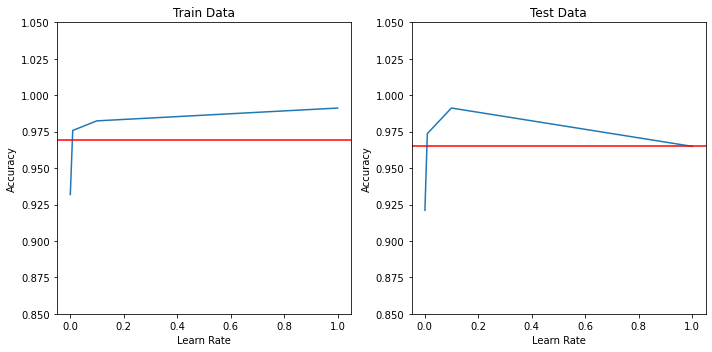
\includegraphics[width=1\linewidth]{Images/epoch100.png}
%     \caption{Accuracy variation as a function of the learning rate for the case with the following hyperparameter: $\lambda=0.001$, batch size=32, epoch=100, test ratio=0.2}
%     \label{fig:epoch100}
% \end{figure}

% In figure \ref{fig:epoch100}the training rate starts to overfit as the learning rate increases, it is evident in the result of the testing accuracy. It is a result of a small number of iteration. One can improve the model by increasing the number of iterations, as seen in the image below the epoch of 1000, which starts performing well as a function of the learning rate.


% \begin{figure}[hbt!]
%     \centering
%     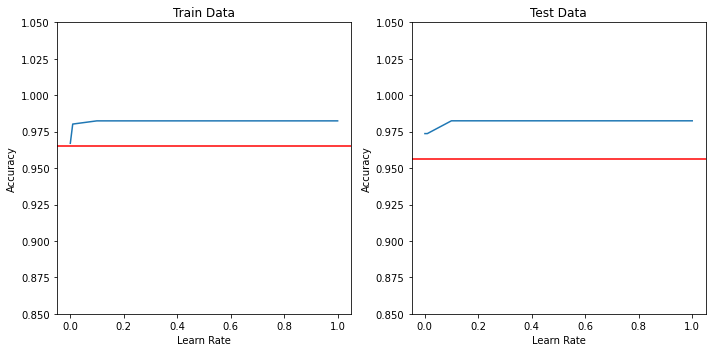
\includegraphics[width=1\linewidth]{Images/epoch1000.png}
%     \caption{Accuracy variation as a function of the learning rate for the case with the following hyperparameter: $\lambda=0.001$, batch size=32, epoch=1000, test ratio=0.2}
%     \label{fig:epoch1000}
% \end{figure}